%!TEX root = ../main.tex
%%%%%%%%%%%%%%%%%%%%%%%%%%%%%%%%%%
% Links: https://www.geeksforgeeks.org/count-pairs-with-given-sum/
% https://algorithms.tutorialhorizon.com/given-an-array-and-a-number-k-check-for-pair-in-array-with-sum-as-k-in-onlgn/
% https://coderbyte.com/algorithm/two-sum-problem https://en.wikipedia.org/wiki/Subset_sum_problem
%
% Difficulty: Easy Companies: Microsoft, Amazon, Google
%%%%%%%%%%%%%%%%%%%%%%%%%%%%%%%%%%

\chapterimage{header} % Table of contents heading image

\chapter{Two numbers sum problem}
\label{ch:two_numbers_sum}
\section*{Introduction}
This chapter addresses one of the most frequently posed problems during the early stages of the coding interview process: two numbers sums.  The problem is hard enough to require non-trivial insights in order to be able to write a non-trivial solution but, at the same time, it is not so hard that it would take a candidate hours to come up with something meaningful to say or to write. It's ubiquity also means that any interviewer will expect a candidate to be at least familiar with the issues and able to present multiple paths to solution. 

We are going to look at several possible solutions.

First, the inefficient brute force approach which we will subsequently refine it into a fast and time-optimal one).
Then,  a radically different approach based on sorting which [AGAIN SOMETHING ABOUT WHY THIS?].
Finally, condensing the strengths of all the previous solutions into a time and space optimal solution that will likely perform best in an interview context. As we will see, this final solution is efficient and not terribly difficult to write and explain; key elements for success in any coding interview.


\section{Problem statement}

\begin{exercise}
	Write a function that takes an array of integers $A$ of size $n$ and an integer $T$, and returns \textbf{true} if the sum of any two distinct elements $I$ is equal to $T$, \textbf{false} otherwise.

	More formally: Given an array $=\{a_1,...,a_n\}$ and $T$, where $a_i, T \in
	\mathcal{N}$, return:
	\begin{itemize}
		\item  \textbf{true} if $\: \exists \;i,j \:\: i \neq j$ s.t. $a_i+a_j = T$
		\item  \textbf{false} otherwise
	\end{itemize}
	

	\begin{example}
	\hfill \\
		Given $A=\{9, 4, 17, 42, 36, -3 ,15\}$ and $T=14$, the function returns \textbf{true} because we can obtain $14$ by summing
		up together the elements $17$ and $-3$.
		If $T=17$ the answer is \textbf{false}.
	\end{example}

	\begin{example}
	\hfill \\
		Given $A=\{1,3,7\}$ and $T=8$, the function returns \textbf{true} because we can obtain $8$ by summing
		up together the elements $7$ and $1$. If $T=6$ the answer is \textbf{false}.
	\end{example}

\end{exercise}	


\section{Clarification Questions}
\begin{QandA}
	\begin{questionitem} \begin{question} Is the input array modifiable?  \end{question} 	 
    \begin{answered}
		\textit{Yes, the input array can be modified.}
	\end{answered} \end{questionitem}	
	\begin{questionitem} \begin{question} Are the integers guaranteed to be all positive or all negative?   \end{question} 	 
    \begin{answered}
		\textit{No, $A$ can contain positive or negative numbers.}
	\end{answered} \end{questionitem}
	\begin{questionitem} \begin{question} Are the values in $A$ guaranteed to be from a given range?  \end{question} 	 
    \begin{answered}
		\textit{No, the input is arbitrary. No assumption can be made on the magnitude of the elements of $A$.}
	\end{answered} \end{questionitem}
	\begin{questionitem} \begin{question} Can a pair be made from an element and itself?  \end{question} 	 
    \begin{answered}
		\textit{No, the pair's elements should be distinct. You cannot use the same element $a_i$ twice. You can however use two elements at indices $i$ and $j$ s.t. $i \neq j$ and $a_i=a_j$.}
	\end{answered} \end{questionitem}
	\begin{questionitem} \begin{question} Are all elements in the array unique?  \end{question} 	 
    \begin{answered}
		\textit{No, duplicates are allowed.}
	\end{answered} \end{questionitem}
	\begin{questionitem} \begin{question} Is the input sorted?  \end{question} 	 
    \begin{answered}
		\textit{No, the ordering of $A$ is arbitrary.}
	\end{answered} \end{questionitem}
	\begin{questionitem} \begin{question} Shall the function integer overflow be considered when performing the sum of two integers? Is it possible for two elements of $A$ to sum up to a value that does not fit in a standard \inline{int}?  \end{question} 	 
    \begin{answered}
		\textit{No, you do not need to worry about overflow.}
	\end{answered} \end{questionitem}
\end{QandA}


\section{Discussion}

%%%%%%%%%%%%%%%%%%%%%%%%%%%%%%%%%%%%%%%
%        quadratic solution
%%%%%%%%%%%%%%%%%%%%%%%%%%%%%%%%%%%%%%
\subsection{Brute-force}
\label{sec:two_numbers:bruteforce}

The brute force solution is straightforward because it consists of a direct application of the formal problem statement. 
The solution space consists of all possible ordered pairs $(a_i,a_j)$, $i < j$. 
Two nested loops can be used to enumerate all those pairs, and, for each of them, we can check whether their sum is equal to $T$: if that is the case,
then   \textbf{true} can be immediately returned, otherwise, if we have checked every possible pair and none of them was good, then we can return  \textbf{false}.
You will find an a fomalization and an implementation of this idea in Algorithm \ref{algo:two_number_sum_bruteforce}
and Listing \ref{list:two_number_sum_bruteforce}), respectively.

\begin{algorithm}
	\SetAlgoLined \SetKwFunction{FMain}{solveQuadratic}
	
	\KwIn{$ A $ \tcp{An array $A$ of length $n$}} \KwIn{$ T $ \tcp{An integer $T$}}

	\Fn{\FMain{$A,T$}}{
	
		%\Output{true if two distinct element of $A$ sum to $T$}
		
		\For{$i\leftarrow 0$ \KwTo $n-1$} {\For{$j\leftarrow i+1$ \KwTo $n$} {\If{$a_i + a_j =
		T$}{\Return True \;}}} \Return False \;}\textbf{End Function}
	
		\caption{Two loops, quadratic solution to the question in Section \ref{ch:two_numbers_sum} }
		\label{algo:two_number_sum_bruteforce}
\end{algorithm}


\lstinputlisting[language=c++, caption="C++ solution of the two number sum problem with a brute force approach.",label=list:two_number_sum_bruteforce]{sources/two_numbers_sum/brute_force.cpp}

The time complexity of this solution is $O(n^2)$ because there is a quadratic number of
ordered pairs and in the worst case, we will look at \textbf{all} of them.

The number of iterations of the internal loop depends on the value of $i$ and
it is described by the function: $f(i) = n-i-1$. The total number of iterations the second
loop runs in the worst case is the the sum of $f(i)$ for all values of $i$: 
$\sum_{i=0}^{n-2} f(i) = (n-1) + (n-2) + (n-3) \ldots + 1 =\sum_{x=1}^{n-1} x= \frac{n(n-1)}{2} = O(n^2)$

The space complexity is $O(1)$.



\subsection{Hashing}
\label{sec:two_numbers:hashing}
The internal loop of the brute force solution above can be eliminated entirely with the help of a hash table.
The key insight is that if a solution exists involving $a_i$ then it must be the case that  exists another element $a_j  = a_i-T$ with $i > j$. 

What this means in practice is that we can loop through $A$ one element at a time and keep track in a lookup table of all the elements seen so far so that the lookup operation for the aforementioned element $a_j$ can be performed in constant time.

Algorithm \ref{algo:two_number_sum_hashset} and Listing \ref{list:two_number_sum_hashing} shows this idea in code.

%%%%%%%%%%%%%%%%%%%%%%%%%%%%%%%%%%%%%%%
% two_numbers_sum_hashset       
%%%%%%%%%%%%%%%%%%%%%%%%%%%%%%%%%%%%%%
\begin{algorithm}
	%	\KwData{} \KwResult{Tr }
	\KwIn{$ A $ \tcp{An array $A$ of length $n$}} \KwIn{$ T $ \tcp{An integer $T$}} \KwOut{true if
	two distinct element of $A$ sum to $T$, False otherwise} \SetKwFunction{FMain}{solveHashSet}
	
    \Fn{\FMain{$A,T$}}{H $\longleftarrow$ \CreateHashSet \;
	
		\For{$i\leftarrow 0$ \KwTo $n$} {target $\leftarrow$ $(T-a_i)$ \eIf{H.find(target)} {\Return
		True} {H.insert($a_i$)}} \Return False\;}\textbf{End Function}

		\caption{Hashset, linear solution to the \textit{two number sum} question in Section
		\ref{ch:two_numbers_sum}.}
		\label{algo:two_number_sum_hashset}
\end{algorithm}


\lstinputlisting[language=c++, caption="C++ solution of the two number sum problem using hashing.",label=list:two_number_sum_hashing]{sources/two_numbers_sum/hashset.cpp}

The time complexity of this approach is $O(n)$ (technically it is linear on average due to the complexity of lookups in hash tables) because the input array is scanned once and for each
of its elements, only one lookup and insertion are performed in the hash table (both operations costing constant time on average).

The space complexity
is also $O(n)$ as, in the worst case scenario,  the whole input array is stored in the lookup table.

A common mistake when solving this problem using this approach is to insert the whole input array into the lookup table, and only after searching for $(T-a_i)$.
The mistake becomes evident when $T$ is an even number ($2 | T$) and $\frac{T}{2}$ appears in $A$  exactly once, at index $k$ i.e. $a_k = \frac{T}{2}$ causing \inline{H.find(T-a_k)} to return \textbf{true}, which is wrong because this corresponds to a solution where we sum $a_k$ twice to obtain $T$.

For instance, when $A=\{1,2,5,4\}$ and $T=10$ this approach wrongly returns \textbf{true}, even if there are not two elements at distinct indices in $A$ whose sum is $T$ (we would use $5$ twice to obtain $10$).
\begin{example}
	\hfill \\ 
	\begin{itemize}
		\item[] $A=\{1,2,5,4\}$
	\item[] $T = 10$
\end{itemize}
	Algorithm \ref{algo:two_numbers_sum_hashset_wrong} wrongly return true even if there are not two
	distinct elements whose sum is $10$.
\end{example}


%%%%%%%%%%%%%%%%%%%%%%%%%%%%%%%%%%%%%%%
% two_numbers_sum_hashset_wrong       
%%%%%%%%%%%%%%%%%%%%%%%%%%%%%%%%%%%%%%
\begin{algorithm}
	\SetKwInOut{Input}{input} \SetKwInOut{Output}{output}
	\SetKwFunction{CreateHashSet}{CreateHashSet<int>} \Input{An array $A$ of length $n$} \Input{An
	integer $T$} \Output{true if two distinct element of $A$ sum to $T$}
	
	\SetKwFunction{FMain}{solveHashSet} \Fn{\FMain{$A,T$}}{H $\longleftarrow$ \CreateHashSet \;
		\tcp{Add the whole array in the hashset}
		\For{$i\leftarrow 0$ \KwTo $n$} {H.insert($a_i$)\;}
		
		\For{$i\leftarrow 0$ \KwTo $n$} {target $\leftarrow$ $T-a_i$ \; \If{H.find(target)} {\Return
		True}} \Return False\;}\textbf{End Function}
		\caption{Hashset, linear solution to the \textit{two number sum} question in Section
		\label{algo:two_numbers_sum_hashset_wrong}
	\ref{ch:two_numbers_sum} }
\end{algorithm}


\subsection{Sorting and binary search}
\label{sect:two_number_problem_binary_search}

As with countless other problems on arrays, sorting the input often leads to a faster and more efficient solution. 

We can start by asking ourselves how the problem changes if  $A$ is sorted. Sorted arrays are naturally associated with binary search as many problems can be solved efficiently by pairing sorting and binary search on arrays. 
This problem is no different therefore we can use binary search if $A$ is sorted to substitute the internal loop of the brute force solution presented [above](). This way, we lower the overall complexity  to $O(n log(n))$; it costs
$O(n log(n))$ to sort the input array in the first place, and the actual search consists of $n$ binary
searches, each of them costing $O(log(n))$. 

The space complexity is $O(1)$ because no additional space is required as the array is sorted in place.

Listing \ref{list:two_number_sum_sorting} shows a C++ implementation of this idea. Note that it uses \inline{std::binary_search} from the C++ standard library and that a possible follow-up question might be to show your own version of the binary search algorithm.



\lstinputlisting[language=c++, caption="C++ solution of the two number sum problem with sorting and binary search.",label=list:two_number_sum_sorting]{sources/two_numbers_sum/two_numbers_sum_sorting.cpp}


\subsection{Sorting and two pointers technique}
\label{sec:two_numbers:twopointers}

There is a variation to the to the approach described in Section
\ref{sect:two_number_problem_binary_search} which still involves sorting but uses a two-pointers
technique instead of binary search to finish the job. 

The key idea is that, once $A$ is sorted, the algorithm initializes
two pointers: one starting at the beginning ($p_s$) and the other at the end ($p_e$) of the array respectively.
It continues by looking at the sum of the two elements pointed by the two pointers and moving one of
the two at each step using the following logic: 
\begin{itemize}
	\item if $a[p_s]+a[p_e] = T$ a solution has been found. The algorithm returns true.
	\item if $a[p_s]+a[p_e] > T$, $p_e=p_e-1$. The right pointer is moved to the left. 
	Moving	$p_e$ to the left has the effect of making the sum of the values pointed by the two pointers smaller (this has an effect at the next iteration). 
	\item if $a[p_s]+a[p_e] < T$, $p_s=p_s+1$. The right end pointer is moved to the left. Moving $p_s$ to the right has the effect of making the sum of the values pointed by the two pointers larger. 
\end{itemize}



Listing \ref{list:two_number_sum_two_pointers} shows an implementation of the idea above. Note that compared to the solution using the binary search, this one is shorter and simpler to write. Moreover, it does not use library functions. 

\lstinputlisting[language=c++, caption="C++ solution of the two number sum problem with the two pointers tecnique.",label=list:two_number_sum_two_pointers]{sources/two_numbers_sum/two_numbers_sum_two_pointers.cpp}

Despite the fact that the overall time complexity is still $O(n log(n))$, this solution is likely to be faster than
using binary search due to the fact that the array is scanned linearly (which makes caches happier) by the two pointers and not in the scattered way of binary search.

%%%%%%%%%%%%%%%%%%%%%
\section*{Variation: Four numbers sum problem}
\label{sec:four_number}

\subsection{Problem statement}

\begin{exercise}
Write a function that takes four arrays of integers, $A,B,C,D$ and a integer $T$,
and returns how many distinct tuple $(i,j,k,l)$ where exist such that $A_i+B_j+C_k+D_l = Y$.

\begin{example}
\hfill \\
Given:
	\begin{itemize}
		\item[-] 	$A=\{1,2\}$,
		\item[-] 	$B=\{-2,-1\}$,
		\item[-] 	$C=\{-1,2\}$,
		\item[-]	$D=\{0,2\}$, and 
		\item[-] 	$T = 0$
	\end{itemize}
The answer is $2$ because the only two valid tuples are:
\begin{enumerate}
	\item $(0,0,0,1)$: $A_0 + B_0 + C_0 + D_1 = 1 + (-2) + (-1) + 2 = T = 0$
	\item $(1,1,0,0)$: $A_1 + B_1 + C_0 + D_0 = 2 + (-1) + (-1) + (-1) = T = 0$
\end{enumerate}
\end{example}
\end{exercise}

\subsection{Na\"ive $O(n^4)$ solution}
We can solve this problem very easily by using the same approach we have described in Section \ref{sec:two_numbers:bruteforce}.
The idea is that we can use four nested loops and enumerate all possible 4-elements tuples of indices. Listing \ref{list:two_number_sum_naive} shows how this can be implemented.
This is not, however,  the fastest solution we can come up with as it has a time complexity of $O(n^4)$

\lstinputlisting[language=c++, caption="Brute force na\"ive solution to the four numbers sum problem.",label=list:two_number_sum_naive]{sources/two_numbers_sum/variations/four_number_sum/four_number_sum_solution1.cpp}

Needless to say, that this is not the fastest solution we can come up with, considering it has a time complexity of $O(n^4)$.

\subsection{$O(n^3)$ solution}
The trivial solution shown in Listing \ref{list:two_number_sum_naive} can be improved by using a similar approach to the one we used to improve the brute-force 
quadratic time solution for the two numbers problem in Listing \ref{list:two_number_sum_bruteforce} and to the linear time (and space) in Listing \ref{list:two_number_sum_hashing}.

The idea is that the inner-most loop is searching for a value $D_l = x$  s.t. if it summed to $A_i+B_j+C_k$ gives us $T$; in other words: $x+(A_i+B_j+C_k)=T$.
Therefore $x = T-(A_i+B_j+C_k)$. If there is a way of avoiding a linear search in the array $D$ for such a value, then we could bring down the complexity from $O(n^4)$ to $O(n^3)$.

This is possible if we use a hash map. If we create a hashmap mapping the value of $D$ and to their frequencies, the inner-most loop of the $O(n^4)$ solution above can be substituted with a query to the hashmap which runs in constant time (on average). 

Listing \ref{list:two_number_sum_cubic} shows an implementation of this idea. 
Note that, in order to obtain the maximum saving in terms of work avoided, the arrays are rearranged in such a way that $D$ is the longest of the four input arrays. 

\lstinputlisting[language=c++, caption="Brute force cubic time solution to the four numbers sum problem.",label=list:two_number_sum_cubic]{sources/two_numbers_sum/variations/four_number_sum/four_number_sum_solution2.cpp}


\subsection{$O(n^2)$ solution using hashing}

This problem can be however be solved  more efficiently in quadratic time if we use hashmaps by holding all  
the frequencies of all the values we can obtain by summing up any two elements of $A$ and $B$ and of $C$ and $D$.
The key idea is that we can build two distinct hashmaps:
\begin{itemize}
	\item $AB$: holding the frequencies of the values obtainable by summing any two elements of $A$ and $B$
	\item $CD$: holding the frequencies of the values obtainable by summing any two elements of $C$ and $D$.
\end{itemize}

The space required for both $AB$ and $CD$ is quadratic, which is more than the space used by any of the previous solutions, but this extra space
also enables us to solve this variation in quadratic time. 

The idea is that we are going to spend $O(n^2)$ time to construct both $AB$ and $CD$
and then again $O(n^2)$ to calculate the final answer 
by searching into $CD$ for the value $T-y$ where $y$ is an element of $AB$. 
If such a value exists in $CD$ it means that there exists one element in  $A$ and one in $B$ such that they sum up to $y$ and
one element $C$ and one in $D$ such that they sum up to $T-y$. Summing all these elements up gives: $y+T-y = T$.
This approach is shown in Listing \ref{list:two_number_sum_quadratic}. 

\lstinputlisting[language=c++, caption="Quadratic time solution to the four numbers sum problem.",label=list:two_number_sum_quadratic]{sources/two_numbers_sum/variations/four_number_sum/four_number_sum_solution3.cpp}

Note that the first thing we do is to fill $AB$ by looping over all possible pairs of elements from $A$ and $B$.
We then do the same thing for $CD$, and finally, in the last loop, we take care of calculating the answer by searching, for each element $(k,v)$ of $AB$, where $k$ is the sum obtained by one element of $A$ and one of $B$, and $v$ is the number of ways we can obtain it,
into $CD$ for the target value $T-k$. If such a value exists into $CD$ then we know we can obtain $T$. The number of times
that is possible is dictated by the frequencies of $k$ and of the target value in $CD$.

However, you might have already noticed that we do not really need to explicitly create the map $CD$. 
When we create $CD$ we already have all the values of $AB$  and therefore for a given $C_i+D_j$ we can already find out how many pairs in $AB$ exist that we can use to get a total sum of $T$. 
This optimization does not really change the overall space complexity
but in practice it means that we use half the memory and we avoid doing $O(n^2)$ work by eliminating the last loop.

Listing \ref{list:two_number_sum_quadratic_opti} shows this optimized version.


\lstinputlisting[language=c++, caption="Space optimized quadratic time solution to the four numbers sum problem.",label=list:two_number_sum_quadratic_opti]{sources/two_numbers_sum/variations/four_number_sum/four_number_sum_solution4.cpp}

%!TEX root = ../main.tex
%%%%%%%%%%%%%%%%%%%%%%%%%%%%%%%%%%
% Links:
%
% Difficulty: Companies: 
%%%%%%%%%%%%%%%%%%%%%%%%%%%%%%%%%%


%\begin{figure} \centering 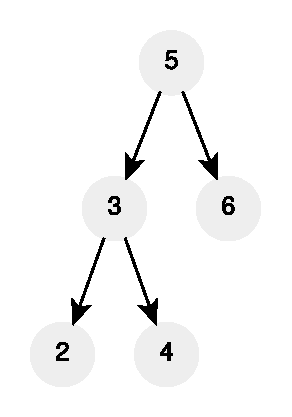
\includegraphics[width=\textwidth]{sources/max_triplet/images/example1}
%   \caption[Sample short cpation]{Sample Caption}. \label{fig:max_triplet:example1} \end{figure}

\section*{Variation: Max triplet sum}
\label{ch:max_triplet}

\subsection{Problem statement}
\begin{exercise}
\label{example:max_triplet:exercice1}
Write a function that, given an array $I$ of length $n$, returns the maximum value obtainable by
summing $3$ distinct elements of $I$: $I_i$, $I_j$ and $I_k$ such that $ 0 \leq i < j < k \leq n-1$
and $ I_i < I_j < I_k $.


	%example1
	\begin{example}
		\label{example:max_triplet:example1}
		\hfill \\
		Given $I = \{2, 5, 3, 1, 4, 9\}$ the function returns $16$. The max value of $16$ is
		obtainable by summing together the elements of $I$ at indices: $0$,$1$ and $5$ : $I_0 +
		I_1+I_5=2+5+9= 16$.
		
		Note that there is another way of obtaining the max sum of $16$; that is by using the
		elements at indices $2$,$4$ and $5$: $I_2 + I_4+I_5=3+4+9= 16$.
	\end{example}

	%example2
	\begin{example}
		\label{example:max_triplet:example2}
		\hfill \\
		Given $I = \{3,2,1\}$ the function returns $-1$ as there is no valid triplet in $I$.		
	\end{example}
	
		\begin{example}
			\hfill \\
			Given $I = \{1,3,2\}$ the function returns $-1$ as there is no valid triplet in $I$.
			\label{ex:max_triplet:example2}	
		\end{example}

	\begin{example}
		\hfill \\
		Given $I = \{1,2,3\}$ the function returns $6$. There is only one valid triplet in $I$.
	\label{ex:max_triplet:example3}
	\end{example}
\end{exercise}

\subsection{Clarification Questions}

\begin{QandA}
	\begin{questionitem} \begin{question} Is it guaranteed that $I$ contains at least three elements?  \end{question} 	 
    \begin{answered}
		\textit{No. When $n < 3$ the function should return $-1$.}
	\end{answered} \end{questionitem}
	\begin{questionitem} \begin{question} Is the answer guaranteed to fit a standard \inline{int}?  \end{question} 	 
    \begin{answered}
		\textit{Yes you can assume the the answer always fits a standard $4$-bytes \inline{int}}
	\end{answered} \end{questionitem}
\end{QandA}

\subsection{Discussion}
\label{max_triplet:sec:discussion}
This problem is asking us to find the largest possible sum obtainable by summing up three distinct
elements of $I$ with the additional constraint that when ordered according to their indices they
form a sorted sequence. You can form such a triplet by selecting an element at index $i$, then
another element at index $j$ that appears after and is larger than the element at index $i$
and finally, a third element at index $k$ which appears after and is larger than the element at
index $j$.

\subsubsection{Brute-force}
\label{max_triplet:sec:bruteforce}
We can solve this problem in a brute-force manner by trying all possible triplets of
ordered indices $i < j <k$ and keeping track of the triplet yielding the maximum value. Three simple
nested loops are enough to implement this idea as shown in Listing
\ref{list:max_triplet_bruteforce}. The time complexity of this approach is $(O(|I|^3)$ which is far
from optimal. The space complexity is $O(1)$ as no additional space is used.

\lstinputlisting[language=c++, caption={Cubic time complexity bruteforce solution.},label=list:max_triplet_bruteforce]{sources/max_triplet/max_triplet_solution1.cpp}


\subsubsection{Pre-calculation and Binary Search}
The cubic time complexity approach discussed in Section \ref{max_triplet:sec:bruteforce} can be
dramatically improved if we approach the problem a little differently. Imagine we would be able to
efficiently calculate $L_j$ and $G_j$ for an element at index $j$ where:
\begin{enumerate}
	\item $L_j$ is the \textbf{largest} value among any of the elements of $I$ appearing at any
	index \textbf{smaller} than $j$ which is \textbf{smaller} than $I_j$;
	\item $G_j$ is the \textbf{largest} value among any of the elements of $I$ appearing at any
	index \textbf{higher} than $j$ which is \textbf{larger} than $I_J$.
\end{enumerate}
When these values are available we can calculate the value of the largest sum obtainable by any
triplet having $I_j$  as the middle element. The triplet $(L_j, I_j, G_j)$ yields the largest sum
as, if that was not the case, it would mean that either a larger element than $L_j$  existed that is also smaller
than $I_j$ in any of the positions before $j$ or that  an element exists that is larger than $G_j$
in any of the positions after $j$. 
Both of these two scenarios are impossible  because $L_j$ is by
definition the largest element that is smaller than $I_j$ and appears before index $j$  and
similarly,  $G_j$ is defined to be the largest element appearing after index $j$ that is larger
than $I_j$.

We can use this fact to calculate the answer to this problem by looping over $I$ and for each
element $I_j$ calculating $L_j+ I_j+ G_j$. The largest of the sums calculated this way is the final
answer. But how can we calculate $L_j$ and $G_j$ for $I_j$?

$L_j$ can be calculated efficiently by keeping a sorted list of all the values appearing before
index $j$ and using binary search to find $L_j$ in the list; while $G_j$ can be pre-calculated using a
similar method as that used to solve the problem in Chapter \ref{ch:greatest_right} where we loop
from the right to the left of $I$ akeep track of the largest element ($M$) seen so far. If $M$ is larger
then the element we are currently examining ($I_x$) then $M$ is also the largest element larger than $I_x$ appearing after $x$.
If not, it means that $I_x$ is the largest element so far and that $I_x$ does not have any larger element on its right: thus $M = I_x$ (see Section \ref{sec:greatest_right:linear} and Listing \ref{list:greatest_right_final1}).
\lstinputlisting[language=c++, caption={$O(nlog(n))$ solution to the max triplet sum problem.},label=list:max_triplet]{sources/max_triplet/max_triplet_solution2.cpp}